Usual quantum information with the usual hindrance of practical implementation.
\begin{parts}
	\part \texttt{NOT}, \texttt{CNOT}, and \texttt{TOFFOLI} are universal in that they are able to replicate a general multi-qubit gate to an arbitrary accuracy.
	
	To construct a \texttt{FREDKIN} gate, we want to have a controlled sequence of \texttt{XOR} gates (i.e. \texttt{CNOT}):
	\begin{figure}[H]
		\centering
		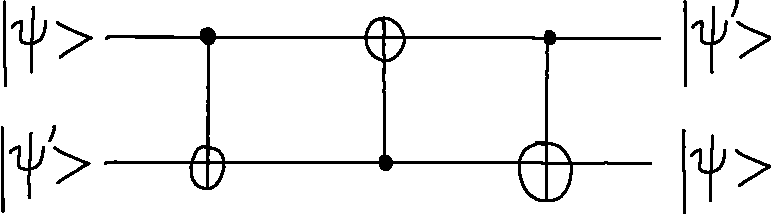
\includegraphics[width=.5\linewidth]{q5-xor}
	\end{figure}
	
	Now realise that \texttt{XOR} is an inverse of itself, we may then replace the central \texttt{CNOT} with \texttt{TOFFOLI}:
	\begin{figure}[H]
		\centering
		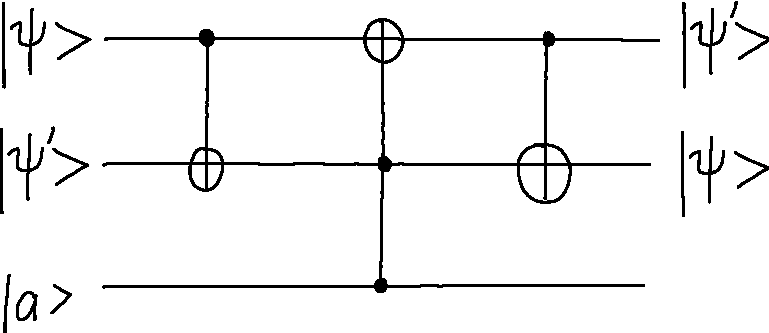
\includegraphics[width=.5\linewidth]{q5-fredkin}
	\end{figure}
	
	Note that if $\ket{a}=\ket{0}$ we have the circuit as \texttt{IDENTITY} and \texttt{SWAP} if $\ket{a}=\ket{1}$.
	
	\part $f: \cbracket{0,\,1}\rightarrow\cbracket{0,\,1}$
	\begin{subparts}
		\subpart There are only 4 such functions:
		
		\begin{tabular}{c|c|c|c|c}
			Input & $f_{00}$ & $f_{01}$ & $f_{10}$ & $f_{11}$ \\ \hline
			0 & 0 & 0 & 1 & 1 \\
			1 & 0 & 1 & 0 & 1 \\ \hline
			& \textbf{constant} & \textbf{balanced} & \textbf{balanced} & \textbf{constant}
		\end{tabular}
		
		\subpart Classically to determine whether $f$ is balanced/constant, we need 2 calls with inputs $\ket{x}=\ket{0}$ and $\ket{x}=\ket{1}$ to obtain the results and compare them against the table above.
		\begin{figure}[H]
			\centering
			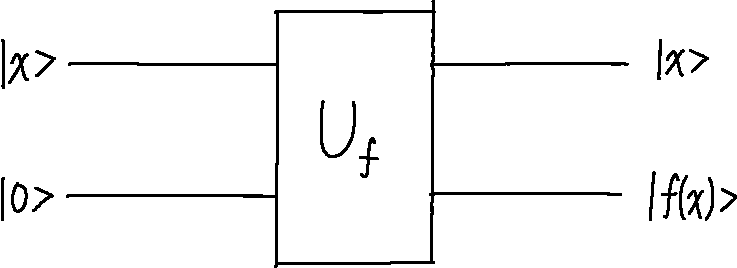
\includegraphics[width=.4\linewidth]{q5-oracle}
		\end{figure}
		\newpage
		Explicit propagator for each $f$:
		\begin{figure}[H]
			\centering
			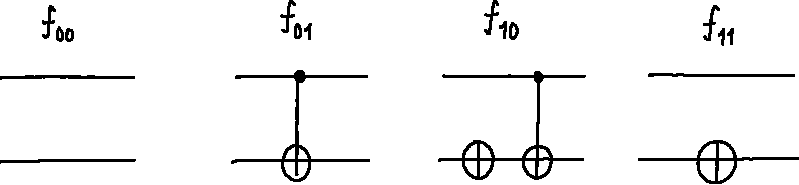
\includegraphics[width=.75\linewidth]{q5-propagator}
		\end{figure}
	\end{subparts}
	
	\part
	Case $f_{00}$:
	\begin{figure}[H]
		\centering
		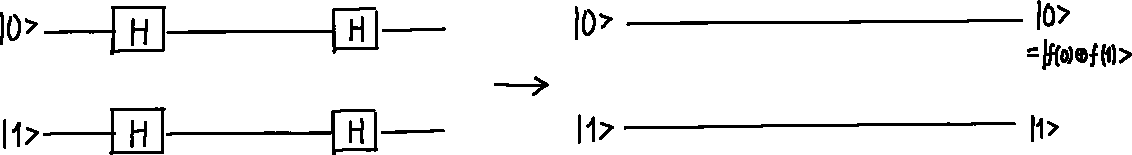
\includegraphics[width=.8\linewidth]{q5-f00}
	\end{figure}
	
	Case $f_{01}$:
	\begin{figure}[H]
		\centering
		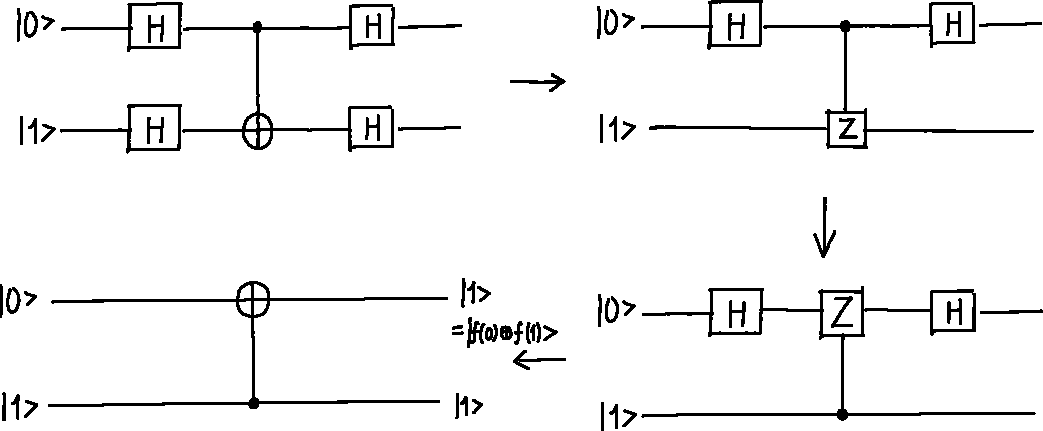
\includegraphics[width=.8\linewidth]{q5-f01}
	\end{figure}
	
	Case $f_{10}$:
	\begin{figure}[H]
		\centering
		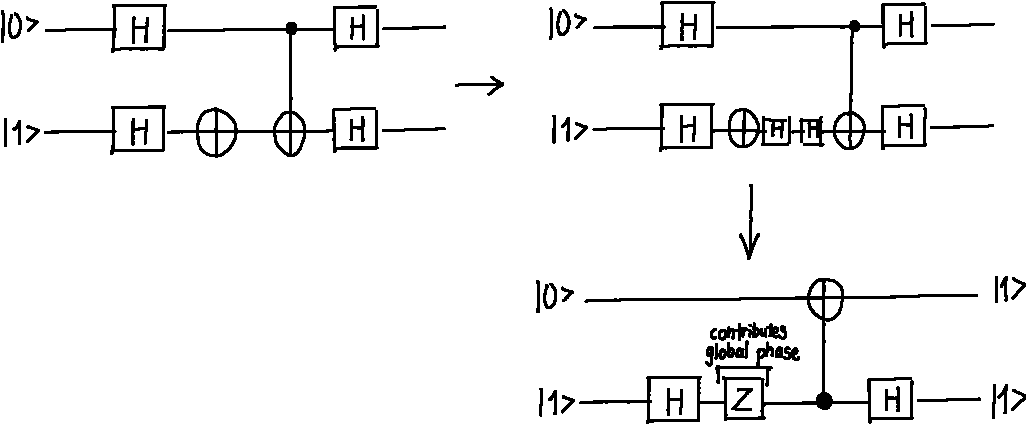
\includegraphics[width=.8\linewidth]{q5-f10}
	\end{figure}
	
	\newpage
	Case $f_{11}$:
	\begin{figure}[H]
		\centering
		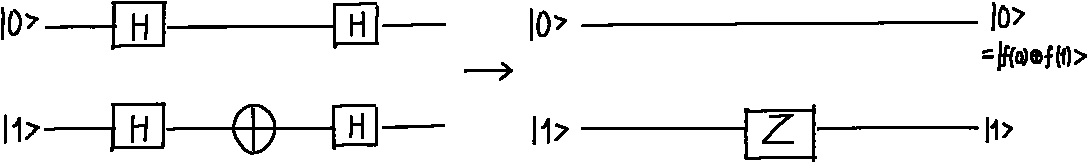
\includegraphics[width=.8\linewidth]{q5-f11}
	\end{figure}
	
	\part \textbf{(DRAFT)} In ion trap computing,
	
	Single-qubit gates: implemented via Rabi flopping -- the pulse time corresponds to the applied phase.
	
	Two-qubit gates: we exploit the cavity condition to achieve 2-qubit manipulation via the long range Coulomb interaction.
	
	\part \textbf{(DRAFT)} For large number of qubits, the Coulomb interaction would inadvertently affect other qubits along the chain of ions, thereby introducing errors to the system.
\end{parts}